\documentclass{article}

\usepackage{geometry}
\usepackage{graphicx}
\usepackage{amsmath}

\title{Database}
\author{Tyler Trogden}

\begin{document}
\maketitle

    \begin{enumerate}
        \item  \textbf{How would you design a database to capture the type of information and data
               in cell-count.csv?}

                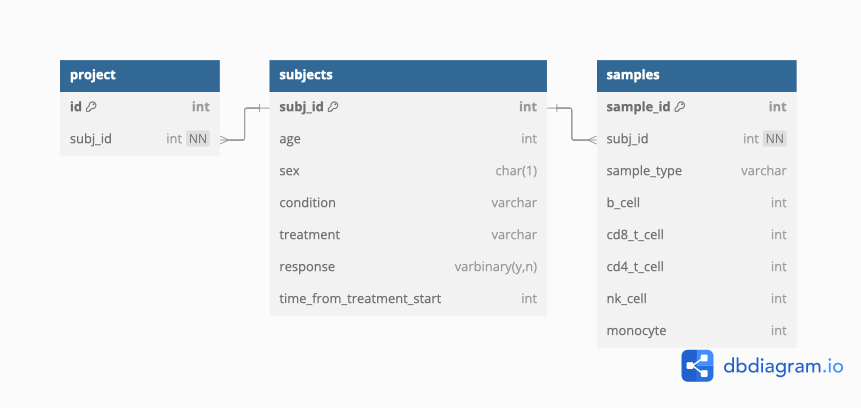
\includegraphics[width=1\textwidth]{db.png}

        \item \textbf{What would be some advantages in capturing this information in a database?}
              Some advantages of capturing this information in a database would be to have
              a structured way to store and query the data, to ensure data integrity, and
              to allow for efficient data retrieval and analysis. Not to mention maintaining
              data security and access control.

        \item \textbf{Based on the schema you provide in (1), please write a query to summarize the number of subjects 
              available for each condition.}

                \begin{verbatim}
                    SELECT condition, COUNT(DISTINCT subj_id) AS num_subj
                    FROM subjects
                    GROUP BY condition;
                \end{verbatim}

        \newpage

        \item \textbf{Please write a query that returns all bladder cancer PBMC samples at baseline
              (\texttt{time\_from\_treatement\_start} is $0$) from patients who have treatment \texttt{tr1}.}
              
                \begin{verbatim}
                    SELECT *
                    FROM samples as smp 
                    WHERE smp.sample_type = `PBMC'
                    LEFT JOIN subjects as sub ON smp.subj_id = sub.subj_id
                    WHERE sub.treatment = `tr1'
                        AND sub.time_from_treatment_start = 0
                        AND sub.condition = `bladder cancer';
                \end{verbatim}

        \item \textbf{Please write queries to provide these following further breakdowns for the samples in (4):}
              Assuming that table \texttt{query as q} is the resultant table from (4).
            \begin{enumerate}
                \item \textbf{How many samples from each project}
                      \begin{verbatim} 
                        SELECT p.id, COUNT(DISTINCT q.sample_id) AS num_samples
                        FROM query as q
                        JOIN project as p ON q.subj_id = p.subj_id
                        GROUP BY p.id;
                      \end{verbatim}

                \item \textbf{How many responders/non-responders}
                      \begin{verbatim}
                        SELECT COUNT(sub.response)
                        FROM subjects as sub
                        JOIN query as q ON sub.subj_id = q.subj_id;
                        GROUP BY sub.response;
                      \end{verbatim}

                \item \textbf{How many males, females}
                      \begin{verbatim}
                        SELECT COUNT(sub.sex)
                        FROM subjects as sub
                        JOIN query as q ON sub.subj_id = q.subj_id
                        GROUP BY sub.sex;
                      \end{verbatim}
            \end{enumerate}
    \end{enumerate}

\end{document}